\section{The effects of fine-tuning and pre-training and on performance and network parameters}
\label{sec:fine}
The results in \cite{Rcnn} (R-CNN) show that supervised pre-training for ImageNet classification followed by fine-tuning for PASCAL object detection leads to large gains over directly using features from the pre-trained network (without fine-tuning).
However, \cite{Rcnn} did not investigate three important aspects of fine-tuning: (1) What happens if we train the network ``from scratch'' (i.e., from a random initialization) on the detection data? (2) How does the amount of fine-tuning data change the picture? and (3) How does fine-tuning alter the network parameters?
In this section, we explore these questions on object detection and image classification datasets.

\subsection{Effect of fine-tuning on performance}
\label{sub:fine-performance}
\setlength{\tabcolsep}{2pt}
\begin{table}[t!]
\begin{center}
\caption{Comparing the performance of CNNs trained from scratch, pre-trained on ImageNet, and fine-tuned. PASCAL-DET+DATA includes additional data from VOC 2012 trainval.}
\vspace{0.3em}
\label{table:fine-effect}
\scalebox{1}{
\begin{tabular}{ccc|ccc|ccc}
\multicolumn{3}{c|}{\textbf{SUN-CLS}} & \multicolumn{3}{c|}{\textbf{PASCAL-DET}} & \multicolumn{3}{c}{\textbf{PASCAL-DET+DATA}} \\
scratch & pre-train & fine-tune  & scratch & pre-train & fine-tune & scratch & pre-train & fine-tune\\
\hline
$40.2 \pm $ & $53.1 \pm 0.2$ & $56.8 \pm 0.2$ & 40.7 & 45.5 & 54.1 & 52.3 & 45.5 & 59.2 \\ 
\end{tabular}}
\end{center}
\end{table}
\setlength{\tabcolsep}{1.4pt}
The main results of this section are presented in Table \ref{table:fine-effect}.
First, we focus on the detection experiments, which we implemented using the open source R-CNN code.
All results use features from layer fc-7.

Somewhat surprisingly, it's possible to get reasonable results (40.7\% mAP) when training the CNN from scratch using only the training data from VOC 2007 trainval (13k bounding box annotations).
Even more surprising is that when the VOC 2007 trainval data is augmented with VOC 2012 data (an additional 25k bounding box annotations), we are able to achieve a mAP of 52.3\% from scratch.
This is almost as good as the performance achieved by pre-training on ImageNet and then fine-tuning on VOC 2007 trainval (54.1\% mAP).
These results can be compared to the 30.5\% mAP obtained by DetectorNet \cite{DetectorNet}, which was trained from scratch on VOC 2012 trainval.

Next, we ask if ImageNet pre-training is still useful in the PASCAL-DET +DATA setting?
Here we see that even though it's possible to get good performance when training from scratch, pre-training still helps considerably.
The final mAP when fine-tuning with the additional detection data is 59.2\%, which is 5 percentage points higher than the best result (without bounding-box regression) reported in \cite{Rcnn}.
This result suggests that R-CNN performance is not data saturated and that simply adding more detection training data without any other changes may substantially improve existing results.

We also present results for SUN image classification.
Here we observe a similar trend: reasonable performance is achievable when training from scratch, however initializing from ImageNet and then fine-tuning yields significantly better performance.

\subsection{Effect of fine-tuning on network parameters}
\label{sub:fine-entropy}
We have provided additional evidence that fine-tuning a discriminatively pre-trained network is very effective in terms of task performance.
Now we look inside the network to see how fine-tuning changes its parameters.

To do this, we define a way to measure the class selectivity of a set of filters.
The precise definition of this measure is given in the supplementary material.
Intuitively, we use the class-label entropy of a filter given its activations on a set of images.
Since this measure is entropy-based, a low value indicates that the filter is highly class selective while a large value indicates that the filter fires regardless of class.

In order to summarize the class selectivity for a \emph{set} of filters, we sort them from the most selective to least selective and plot the average selectivity of the first $k$ filters while sweeping $k$ down the sorted list.
Figure \ref{fig:fine-entropy} shows the class selectivity for the sets of filters in layers 1 to 7 before and after fine-tuning (on VOC 2007 trainval).
Selectivity is measured using the ground truth boxes from PASCAL-DET-GT instead of a whole-image classification task to ensure that filter responses are a direct result of the presence of object categories of interest and not correlations with image background.

\begin{comment}
\begin{figure}[t!]
\centering
\subfloat{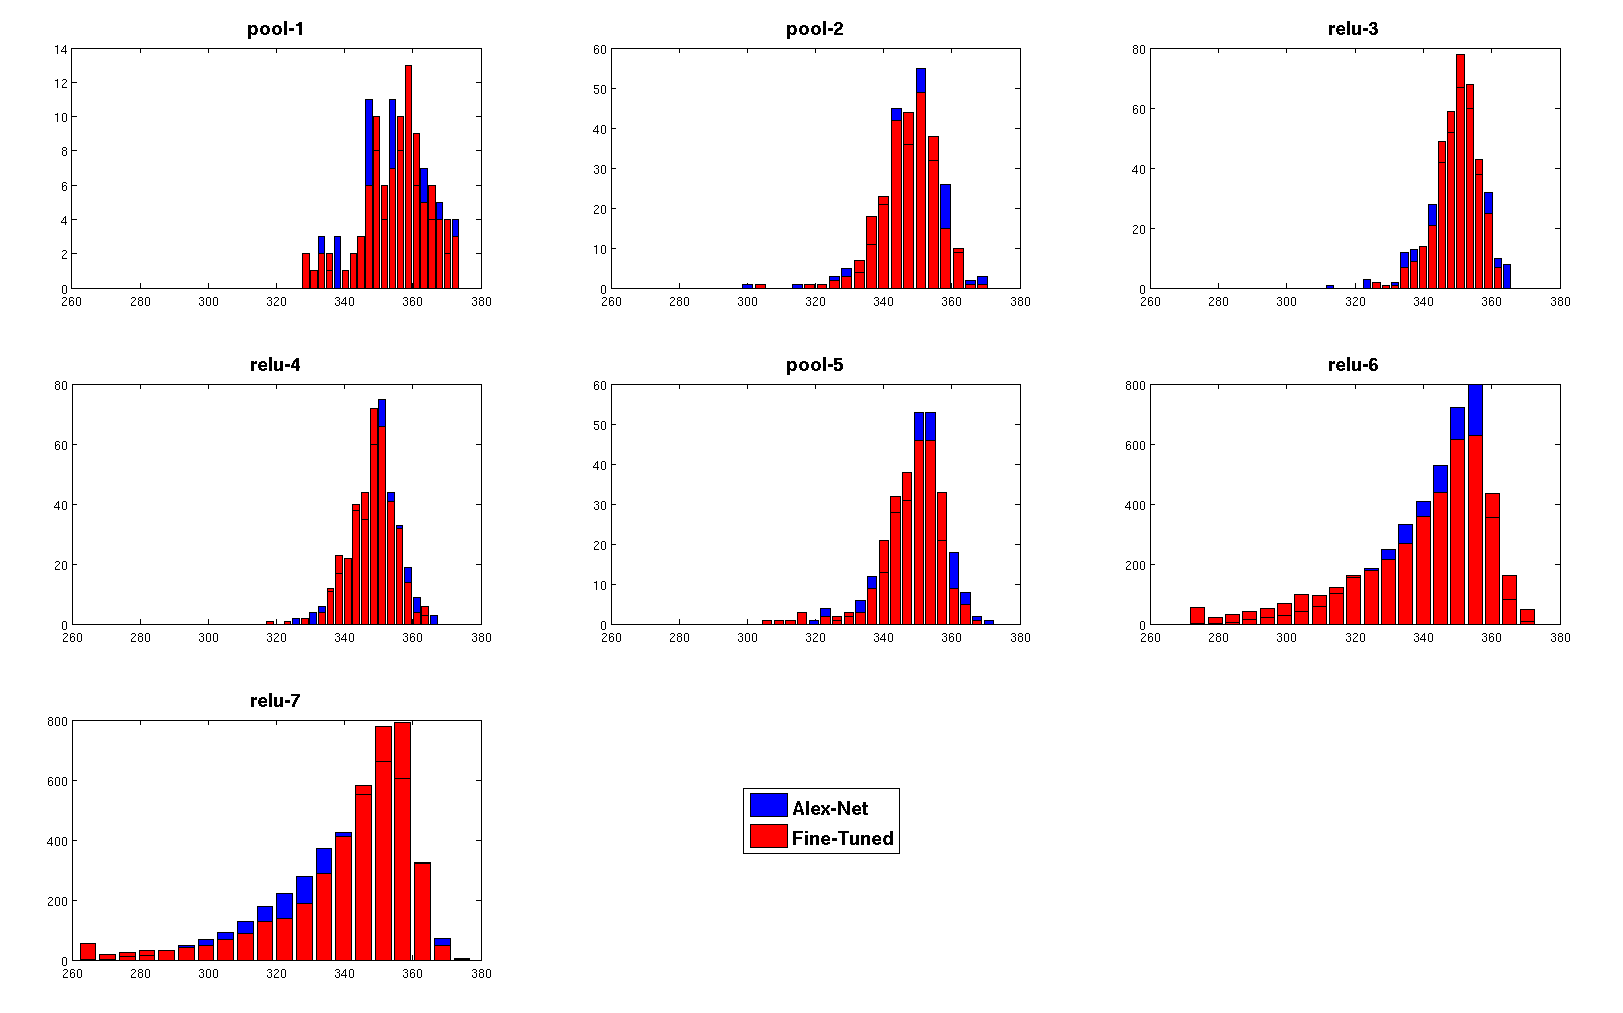
\includegraphics[height=6.5cm]{images/ent_hist.png}}
\caption{Distribution of AuE for different layers in Alex-Net and FT-Net. X-axis is the entropy and the Y-axis is the number of filters. Notice that the left tail for fc-6 and fc-7 becomes heavier after finetuning. This indicates that finetuning makes these filters more discriminative.}
\label{fig:fine-hist}
\end{figure}
\end{comment}

\begin{figure}[t!]
\centering
\subfloat{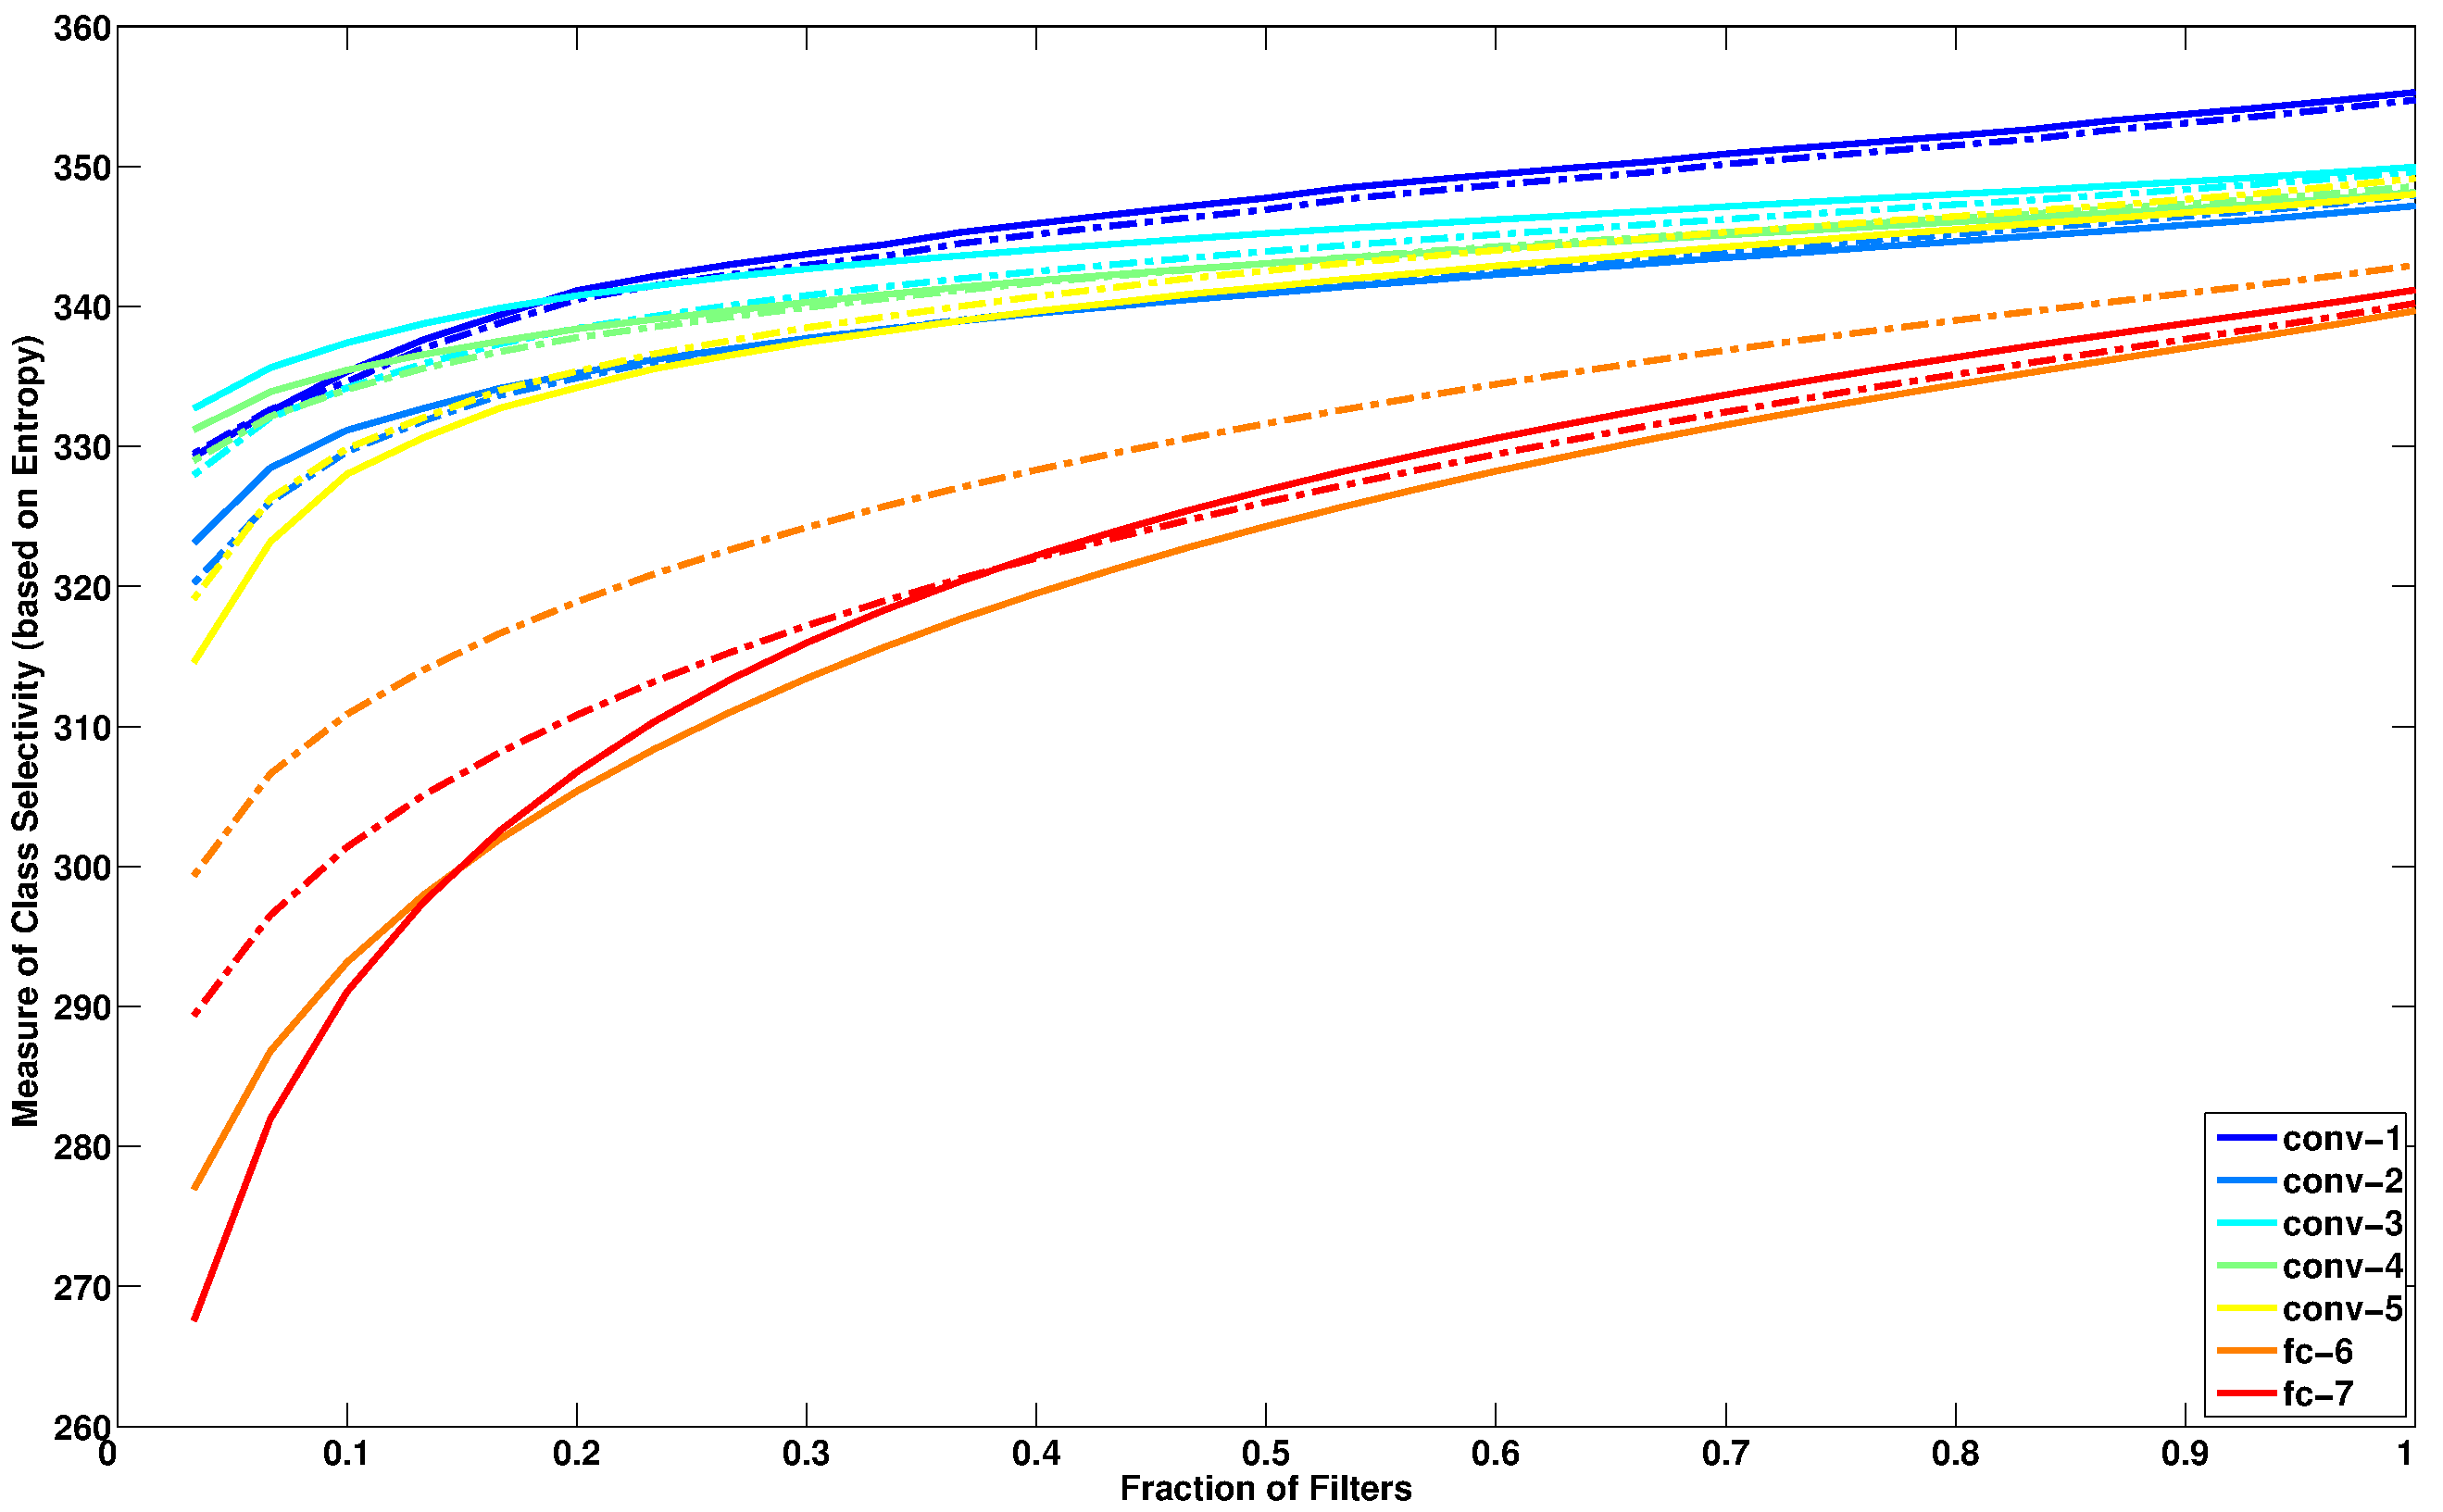
\includegraphics[scale=0.20]{images/MCAUE.pdf}}
\caption{Class selectivity plotted against the fraction of filters for all layers of  (dash-dot line) and a fine-tuned network (solid line). A lower value indicates that the layer is more class selective. Although layers become more discriminative as we go higher up in the network (i.e. from layer 1 to 7), fine-tuning on limited data (PASCAL-DET) only seems to significantly effect the last two layers.}
\label{fig:fine-entropy}
\end{figure}

\setlength{\tabcolsep}{2pt}
\begin{table}[t!]
\begin{center}
\caption{Comparison in performance when fine-tuning the entire network (ft) versus only fine-tuning the fully-connected layers (fc-ft).}
\label{table:fine-fc-ft}
\vspace{0.3em}
\scalebox{1}{
\begin{tabular}{cc|cc|cc}
\multicolumn{2}{c|}{\textbf{SUN-CLS}} & \multicolumn{2}{c|}{\textbf{PASCAL-DET}} & \multicolumn{2}{c}{\textbf{PASCAL-DET+DATA}} \\
ft & fc-ft  & ft & fc-ft & ft & fc-ft \\
\hline
$56.8 \pm 0.2$ & $56.2 \pm 0.1$ & 54.1 & 53.3 & 59.2 & 56.0 \\ 
\end{tabular}}
\end{center}
\end{table}
\setlength{\tabcolsep}{1.4pt}

Figure \ref{fig:fine-entropy} shows that class selectivity increases from layer 1 to 7 for both networks.
This result is consistent with performance numbers reported in Table \ref{table:det-traj-classify}. 
However, it is interesting to note that entropy changes due to fine-tuning are only significant for layers 6 and 7. 
This observation indicates that fine-tuning only layers 6 and 7 may suffice for achieving good performance when fine-tuning data is limited. 
We test this hypothesis on SUN-CLS and PASCAL-DET by comparing the performance of a fine-tuned network (ft) with a network which is fine-tuned by only updating weights of fc-6 and fc-7 (fc-ft network). 
Results are summarized in Table \ref{table:fine-fc-ft}.
With small amounts of data, fine-tuning amounts to ``rewiring'' the fully connected layers.
However, when more fine-tuning data is available (PASCAL-DET+DATA), there is still substantial benefit from fine-tuning all network parameters.

%We find that the final performance in the detection setup only drops by 0.8 points and by 0.6 points for scene-classification.  

%\setlength{\tabcolsep}{1pt}
%\begin{table}[t!]
%\begin{center}
%\caption{\todo{Include layer-wise results for PASCAL-DET-2?} for Evaluation of effect finetuning towards the task of object detection. (l5, l6, l7: layers 5, 6 and 7 of Alex Net)}
%\label{table:det-fine}
%\scalebox{0.75}{
%\begin{tabular}{l|cccccccccccccccccccc||c}
%\hline\noalign{\smallskip}
%layer & aero & bike & bird & boat & bottle & bus & car & cat & chair & cow & table & dog & horse & mbike & person & plant & sheep & sofa & train & tv & mAP \\
%\noalign{\smallskip}
%\hline
%l5 & 51.9 & 61.1 & 36.8 & 28.4 & 23.7 & 52.3 & 60.8 & 48.4 & 24.9 & 47.1 & 47.5 & 42.1 & 55.6 & 58.7 & 42.5 & 24.5 & 46.9 & 39.3 & 52.0 & 55.4 & 45.0 \\
%l5-ft & 57.8 & 63.9 & 38.8 & 28.0 & 29.0&54.8&66.9&51.3 & 30.5 & 52.1 & 45.2 & 43.2 & 57.3 & 58.8 & 46.0 & 27.2 & 51.2 & 39.3 & 53.3 & 56.6 & 47.6 \\
%\hline 
%l6-ft &63.5 & 66.3 & 48.7 & 38.1 & 30.6 & 61.4 & 70.9 & 60.3 & 34.8 & 57.8 & 47.6 & 53.6 & 59.8 & 63.5 & 52.5 & 29.8 & 54.6 & 48.2 & 58.5 & 62.2 & 53.1 \\
%l6-fc-ft& 61.4 & 63.9 & 44.2 & 36.2 & 29.0 & 59.9 & 66.0 & 55.3 & 31.1 & 57.6 & 49.5 & 49.4 & 59.4 & 63.7 & 50.8 & 29.5 & 54.1 & 43.2 & 57.4 & 58.8 & 51.0 \\
%\hline
%l7 & 57.6 & 57.2 & 41.4 & 31.2 & 25.6 & 52.4 & 58.8 & 50.9 & 25.2 & 50.4 & 42.7 & 47.1 & 52.2 & 55.6 & 44.5 & 23.9 & 48.0 & 38.1 & 51.5 & 56.6 & 45.5 \\
%l7-ft & 64.3 & 69.6 & 50.1 & 41.8 & 32.0 & 62.6 & 71.0 & 60.6 & 32.8 & 58.5 & 46.4 & 56.0 & 60.0 & 66.9 & 54.2 & 31.5 & 52.7 & 48.8 & 57.7 & 64.7 & 54.1 \\
%l7-fc-ft & 62.9 & 65.2 & 47.5 & 39.0 & 30.3 & 63.1 & 68.4 & 59.7 & 34.2 & 58.5 & 52.0 & 53.8 & 60.7 & 65.3 & 53.0 & 30.2 & 55.5 & 46.3 & 57.7 & 62.2 & 53.3 \\
%\hline
%\end{tabular}}
%\end{center}
%\end{table}
%\setlength{\tabcolsep}{1.4pt}

%A detailed layer-wise analysis of detection performance for all PASCAL classes and the 3 network configurations is presented in table \ref{table:det-fine}. %
%Notice that for both the finetuned networks there is big jump in the performance while going from layer 5 to 6 and a rather small jump from layer 6 to 7. For Alex-Net, the performance is virtually the same for layers 5 and 7. It is also notable, that although the performance for FT-net is better by 2.6 points at layer 5 - the performance is virtually the same at layer 7. 

%\subsection{Discussion}
%\label{sub:fine-discussion}
%Since layers 1-5 change a little over the course finetuning, this suggests that these are generic features. 
%
%%Although, one could always improve performance by a few points by finetuning the full network - for a lot of applications this may not be practical. 
%
%\todo{Talk about the entropy metric with respect to code being distributed.}
%
%\todo{Side Note - may or may not include}In our experiments we also noted accuracy of image classification on PASCAL is almost untouched by finetuning. This is suggestive of the fact finetuning is a task specific operation and finetuning for detection does not necessarily leads to an increase in classification performance, even though the classes and images are shared across PASCAL classification and detection challenges.

\subsection{Effect of pre-training on network parameters}
\label{sec:speed}
\section{How does pre-training time effect generalization performance?}
\label{sec:speed}
%Pre-Training is the process of initializing CNN parameters for a target application using images from a (generally larger) separate dataset. Features learned by a CNN pre-trained on Imagenet have been shown to generalize and achieve state of art results across multiple computer vision datasets (see section \ref{sec:fine} and \cite{Decaf}). Since, no single image dataset fully captures the variation in natural images, all datasets are biased (cite Alyosha). Consequently, it can be expected that excessive pre-training can cause the CNN to overfit on Imagenet and thus hurt generalization performance. 
There is no single image dataset which fully captures the variation in natural images. This means that all datasets including Imagenet are biased (cite Alyosha). Thus, there is a possibility that excessive pre-training can cause the CNN to overfit and consequently hurt generalization performance. Therefore, we need to investigate the effect of pre-training time on generalization performance.

We studied the effect of pre-training time under two experimental setups. In the first, we directly measured  the performance of features extracted from a CNN pre-trained on Imagenet as a function of number of pre-training iterations (see table \ref{table:det-traj-classify}). In the second, we fine-tuned the CNN after different number of pre-training iterations  for SUN-CLS and PASCAL-DET after pre-training for different number of 

In order to determine if this is indeed the case, we analysed the performance of features extracted  at various time steps from a network trained on Imagenet for classifying images on the PASCAL-2007 dataset. Linear SVMs were trained for classification and the results are presented in table \ref{table:det-traj-classify}. It is quite surprising to note that by 15K iterations all layers are within 80\% and at 50K iterations within 90\% of there final performance. This strongly indicates that a great portion of training required for generalization happens quite quickly. 


\setlength{\tabcolsep}{4pt}
\begin{table}[t!]
\begin{center}
\caption{Variation in classification accuracy (mean-AP) on PASCAL-2007 challenge using features extracted from different layers of Alex-Net as a function of number of iterations.}
\label{table:det-traj-classify}
\begin{tabular}{lcccccccccc}
\hline\noalign{\smallskip}
Layer  & 5K & 15K & 25K & 35K & 50K & 95K & 105K & 195K & 205K & 305K \\
\noalign{\smallskip}
\hline
\noalign{\smallskip}
conv-1 & 23.0 & 24.3 & 24.4 & 24.5 & 24.3 & 24.8 & 24.7 & 24.4 & $24.4 \pm 0.5$ & -\\
conv-2 & 33.7 & 40.4 & 40.9 & 41.8 & 42.7 & 43.2 & 44.0 & 45.0 & $45.1 \pm 0.7$ & -\\
conv-3 & 34.2 & 46.8 & 47.0 & 48.2 & 48.6 & 49.4 & 51.6 & 50.7 & $50.9 \pm 0.6$ & -\\
conv-4 & 33.5 & 49.0 & 48.7 & 50.2 & 50.7 & 51.6 & 54.1 & 54.3 & $54.4 \pm 0.6$ & -\\
conv-5 & 33.0 & 53.4 & 55.0 & 56.8 & 57.3 & 59.2 & 63.5 & 64.9 & $65.5 \pm 0.3$ & -\\
fc-6 & 34.2 & 59.7 & 62.6 & 62.7 & 63.5 & 65.6 	& 69.3 & 71.3 & $71.8 \pm 0.3$ & -\\
fc-7 & 30.9 & 61.3 & 64.1 & 65.1 & 65.9 & 67.8 	& 71.8 & 73.4 & $74.0 \pm 0.3$ & -\\
\hline
\end{tabular}
\end{center}
\end{table}
\setlength{\tabcolsep}{1.4pt}

\begin{figure}[t!]
\centering
\subfloat[5K Iterations]{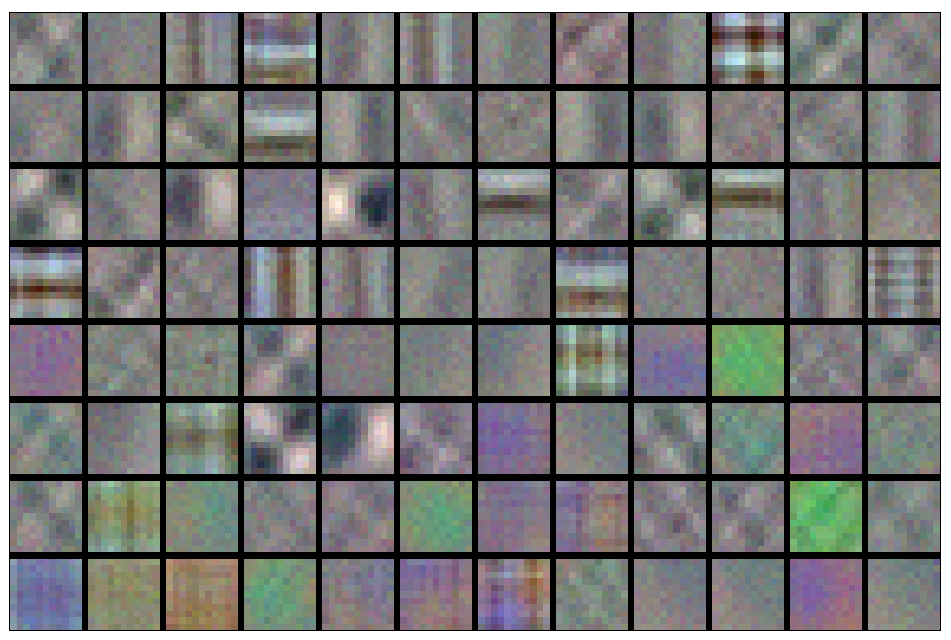
\includegraphics[scale=0.10]{images/l1_filters_iter5000.png}} \hspace{2mm}
\subfloat[15K Iterations]{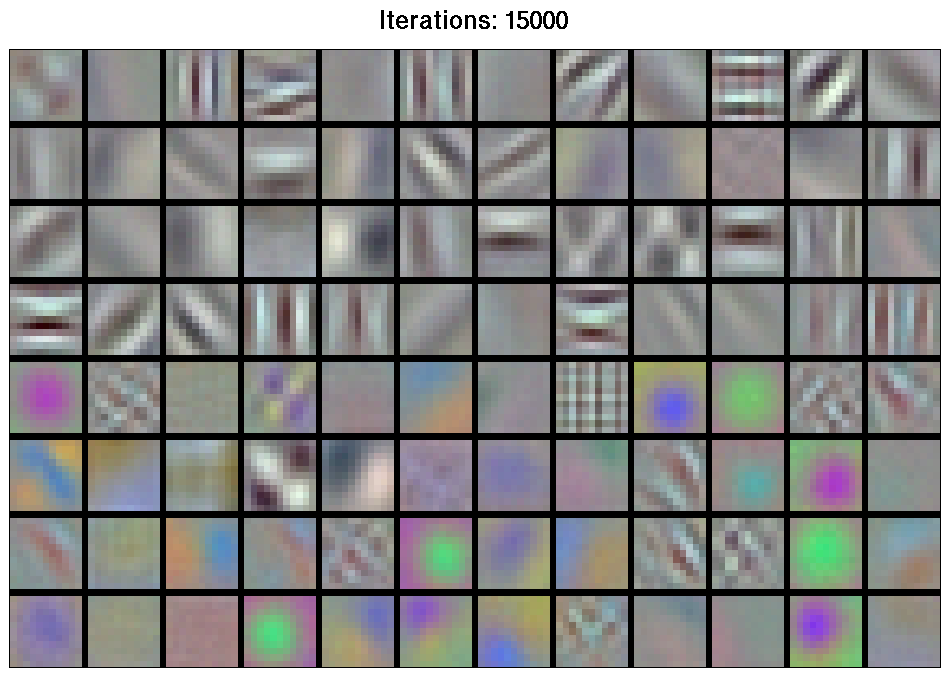
\includegraphics[scale=0.10]{images/l1_filters_iter15000.png}} \hspace{2mm}
\subfloat[305K Iterations]{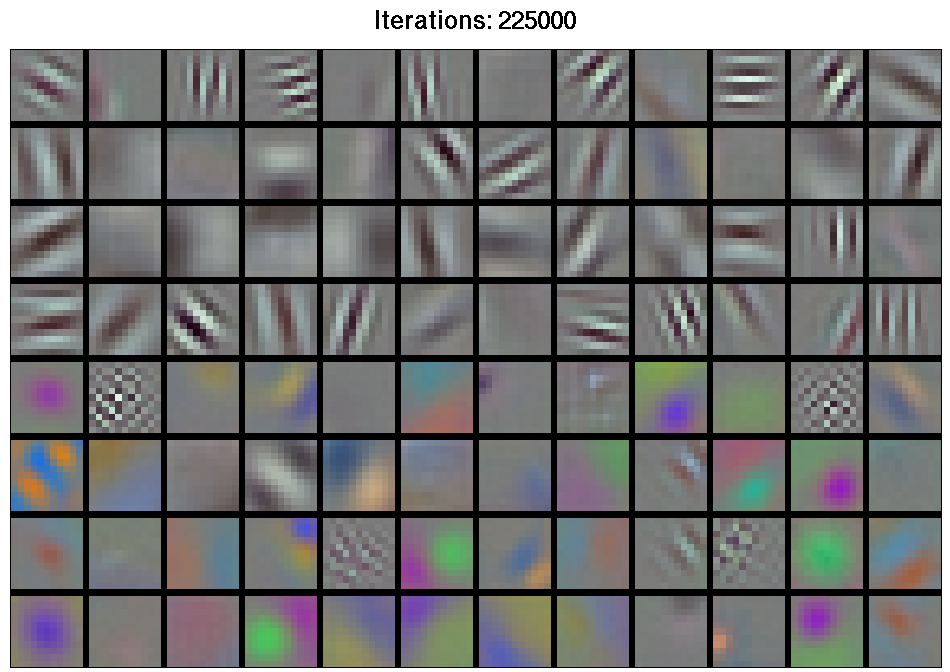
\includegraphics[scale=0.10]{images/l1_filters_iter225000.png}}
\caption{(a),(b),(c) show conv-1 filters after 5K, 15K and 305K iterations of training respectively. One pass (epoch) over the entire Imagenet-ILSVRC12 dataset takes approximately 5K iterations. Notice, that just after 15K iterations these filters closely resemble their final state.}
\begin{comment} Note: I have labeled 305K as 225K - I cannot get the same shape as of the 5K,15K for 305K. The filters look very similar and visually indistiguishable from 305K. If I have time later, I will make them all uniform.
\end{comment}
\label{fig:conv1}
\end{figure}


\setlength{\tabcolsep}{1pt}
\begin{table}[t!]
\begin{center}
\caption{Performance of 50-50 network for detection on pascal-voc-2007 challenge. (l5 is conv-5 and l7 is fc-7)}
\label{table:det-trajectory}
\scalebox{1.00}{
\begin{tabular}{|l|cccc|}
\hline
 & 50K & 105K & 205K & 305K \\
\hline
PASCAL-DET & 50.2 & 52.6 & 55.3 & 55.4 \\
SUN-CLS & 52.8 & 54.7 & 56.4 & 56.6 \\
\hline
\end{tabular}}
\end{center}
\end{table}
\setlength{\tabcolsep}{1.4pt}
The above analysis reinforces our belief that indeed majority of training required for generalization happens quite quickly as compared to the full training time of the network. This observation suggest that there may exist clever ways which can help us speed up the training.


